%%%%%%%%%%%%%%%%%%%%%%%%%%%%%%%%%%%%%%%%%
% Beamer Presentation
% LaTeX Template
% Version 1.0 (10/11/12)
%
% This template has been downloaded from:
% http://www.LaTeXTemplates.com
%
% License:
% CC BY-NC-SA 3.0 (http://creativecommons.org/licenses/by-nc-sa/3.0/)
%
%%%%%%%%%%%%%%%%%%%%%%%%%%%%%%%%%%%%%%%%%

%----------------------------------------------------------------------------------------
%	PACKAGES AND THEMES
%----------------------------------------------------------------------------------------

\documentclass{beamer}

\mode<presentation> {

% The Beamer class comes with a number of default slide themes
% which change the colors and layouts of slides. Below this is a list
% of all the themes, uncomment each in turn to see what they look like.

%\usetheme{default}
%\usetheme{AnnArbor}
%\usetheme{Antibes}
%\usetheme{Bergen}
%\usetheme{Berkeley}
%\usetheme{Berlin}
%\usetheme{Boadilla}
%\usetheme{CambridgeUS}
%\usetheme{Copenhagen}
%\usetheme{Darmstadt}
%\usetheme{Dresden}
%\usetheme{Frankfurt}
%\usetheme{Goettingen}
%\usetheme{Hannover}
%\usetheme{Ilmenau}
%\usetheme{JuanLesPins}
%\usetheme{Luebeck}
%\usetheme{Madrid}
%\usetheme{Malmoe}
%\usetheme{Marburg}
\usetheme{Montpellier}
%\usetheme{PaloAlto}
%\usetheme{Pittsburgh}
%\usetheme{Rochester}
%\usetheme{Singapore}
%\usetheme{Szeged}
%\usetheme{Warsaw}

% As well as themes, the Beamer class has a number of color themes
% for any slide theme. Uncomment each of these in turn to see how it
% changes the colors of your current slide theme.

%\usecolortheme{albatross}
%\usecolortheme{beaver}
%\usecolortheme{beetle}
%\usecolortheme{crane}
%\usecolortheme{dolphin}
%\usecolortheme{dove}
%\usecolortheme{fly}
\usecolortheme{lily}
%\usecolortheme{orchid}
%\usecolortheme{rose}
%\usecolortheme{seagull}
%\usecolortheme{seahorse}
%\usecolortheme{whale}
%\usecolortheme{wolverine}

%\setbeamertemplate{footline} % To remove the footer line in all slides uncomment this line
%\setbeamertemplate{footline}[page number] % To replace the footer line in all slides with a simple slide count uncomment this line

%\setbeamertemplate{navigation symbols}{} % To remove the navigation symbols from the bottom of all slides uncomment this line
}
\usepackage{algorithm}
\usepackage{algorithmic}
\usepackage{graphicx} % Allows including images
\usepackage{booktabs} % Allows the use of \toprule, \midrule and \bottomrule in tables

%----------------------------------------------------------------------------------------
%	TITLE PAGE
%----------------------------------------------------------------------------------------

\title[Euclidean Algorithm]{Exploring the Euclidean Algorithm} % The short title appears at the bottom of every slide, the full title is only on the title page

\author{Stephen Capps, Sarah Sahibzada, \& Taylor Wilson} % Your name
\institute[TAMU] % Your institution as it will appear on the bottom of every slide, may be shorthand to save space
{
Texas A\&{}M University \\ % Your institution for the title page
\medskip
\textit{Supurvisor: Sara Pollock} % Your email address
}
\date{\today} % Date, can be changed to a custom date

\begin{document}

\begin{frame}
\titlepage % Print the title page as the first slide
\end{frame}

\begin{frame}
\frametitle{Overview} % Table of contents slide, comment this block out to remove it
\tableofcontents % Throughout your presentation, if you choose to use \section{} and \subsection{} commands, these will automatically be printed on this slide as an overview of your presentation
\end{frame}

%----------------------------------------------------------------------------------------
%	PRESENTATION SLIDES
%----------------------------------------------------------------------------------------

%------------------------------------------------
\section{Introduction}
\subsection{Definition}
\begin{frame}
\frametitle{The Euclidean Algorithm} $ $
\indent The Euclidean Algorithm is used to find the Greatest Common Divisor between any pair of whole numbers $\mathrm{p, q}$ such that $\mathrm{p>q}$.
\indent It follows that 
$$p = n_1*q + r_1$$ 
$$q = n_2*r_1 + r_2$$
$$.$$
$$.$$
$$.$$
$$r_{k-1} = n_{k+1}*r_k$$
Where \begin{center}$r_k = \mathrm{gcd(p,q)}$.\end{center}
\end{frame}
\subsection{Examples}
\begin{frame}
For example, here is the gcd$(42,36)$:
		$$\mathrm{gcd}(42,36) = 6:$$

\begin{center}--------------------------------------------------------------
\end{center}	
	\begin{equation}
		42 = 1 * 36 + 6
	\end{equation}
	\begin{equation}
		36 = 6 * 6 + 0
	\end{equation}
As you can see, it took $2$ iterations to complete the algorithm. This is what we will explore. Here are some more gcds and their iterations:

\begin{center}
\begin{tabular}{c|c}

$\mathrm{gcd}(\mathrm{p},\mathrm{q}) = \mathrm{d}$ & Iterations
\\
\hline
$\mathrm{gcd}(689,456) = 1$ & $6$\\

$\mathrm{gcd}(78,45) = 3$ & $5$\\

$\mathrm{gcd}(8394,238) = 2$ & $7$\\


\end{tabular}
\end{center}
\end{frame}

\section{Euclidean Algorithm Iterations and Results}

\subsection{What to explore}
\begin{frame}
Next, we decided to explore the distributions of these iterations:
Do most pairs take many iterations? What is the distribution?

The following graphs are the answer to these questions.


\end{frame}
\subsection{Distribution Results}
\begin{frame}
\begin{figure}
		
		\center 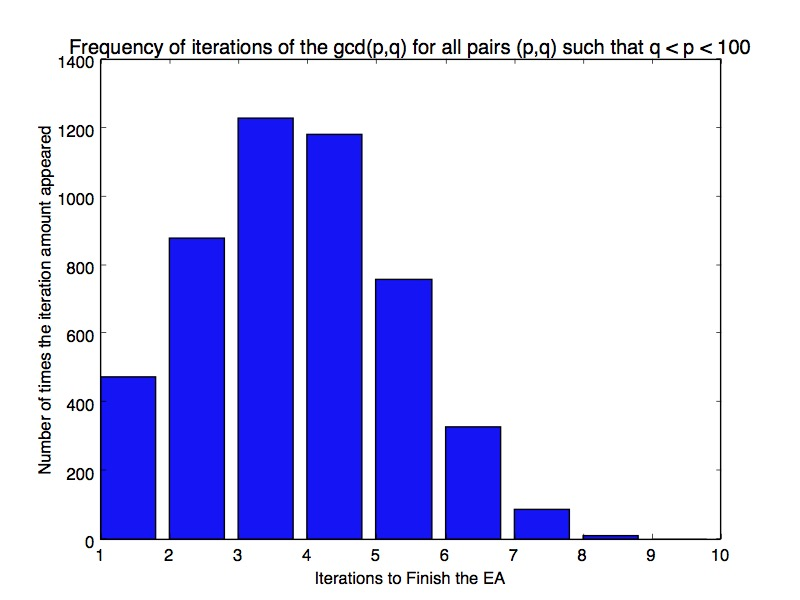
\includegraphics[scale=.3]{2digit_iterationfreq.jpg}
		\center \tiny(Figure 1)
\end{figure}


\end{frame}

\begin{frame}
\begin{figure}
		
		\center 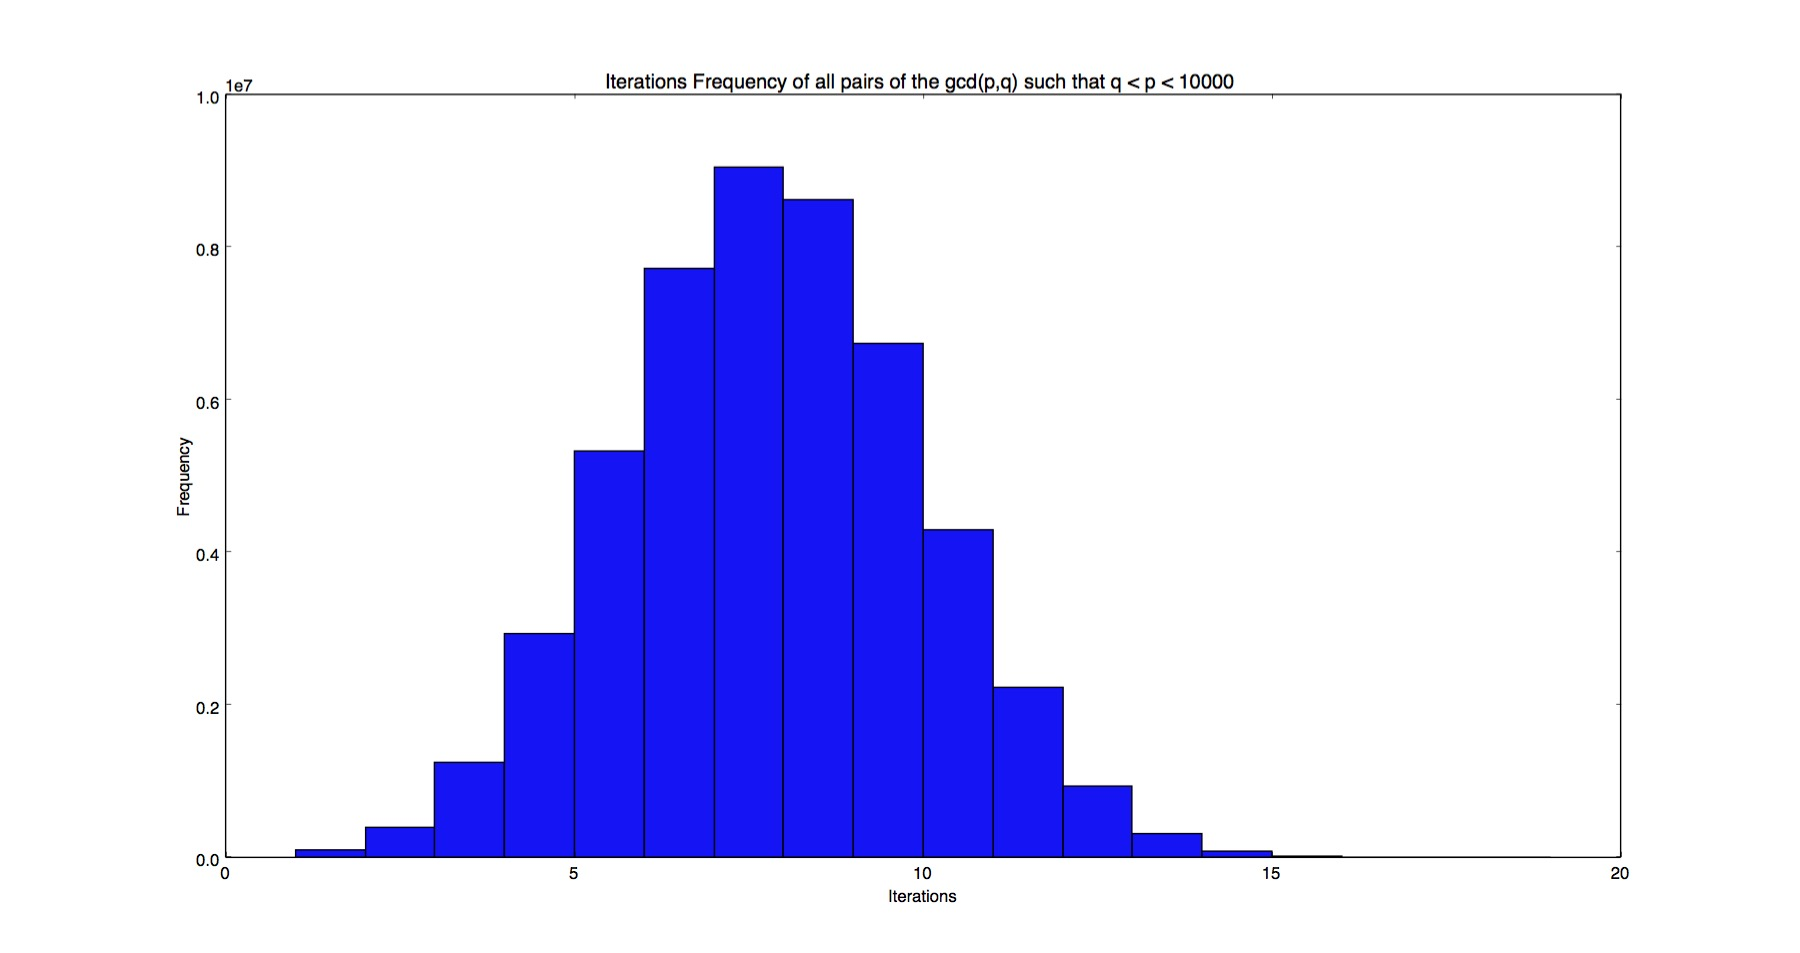
\includegraphics[scale=.3]{4digit_iteration_freq.jpg}
		\center \tiny(Figure 2)
\end{figure}


\end{frame}

\begin{frame}
\begin{figure}
		
		\center 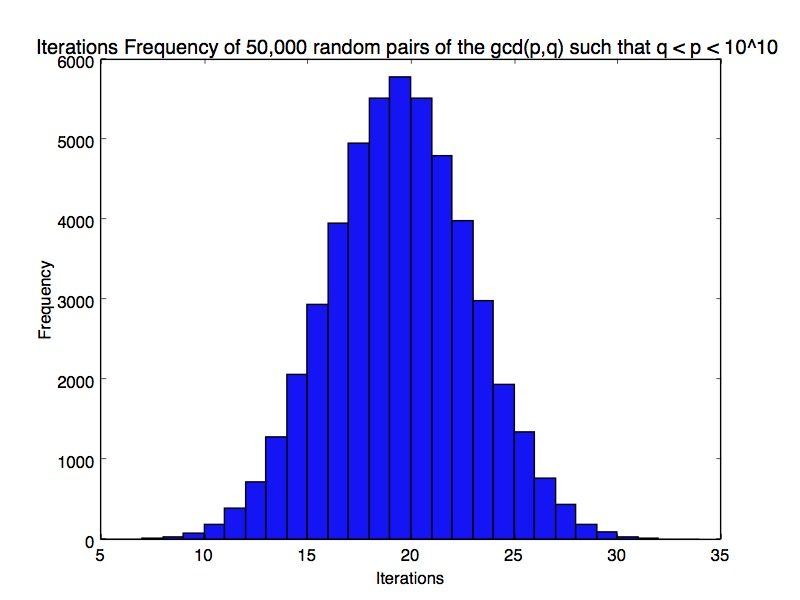
\includegraphics[scale=.3]{10_digit_numbers.jpg}
		\center \tiny(Figure 3)
\end{figure}

\end{frame}

\begin{frame}
		\center 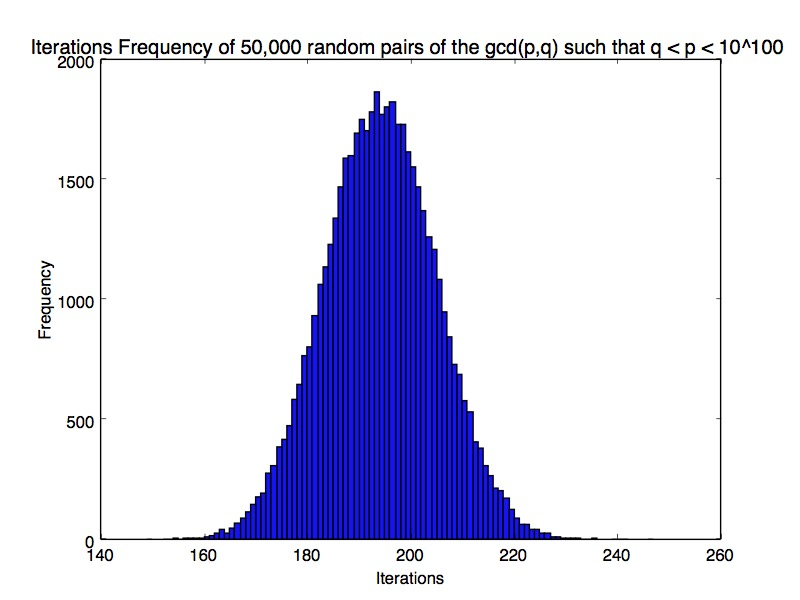
\includegraphics[scale=.3]{100_digit_numbers_freq.jpg}
		\center \tiny(Figure 4)

\end{frame}

\begin{frame}
		\center 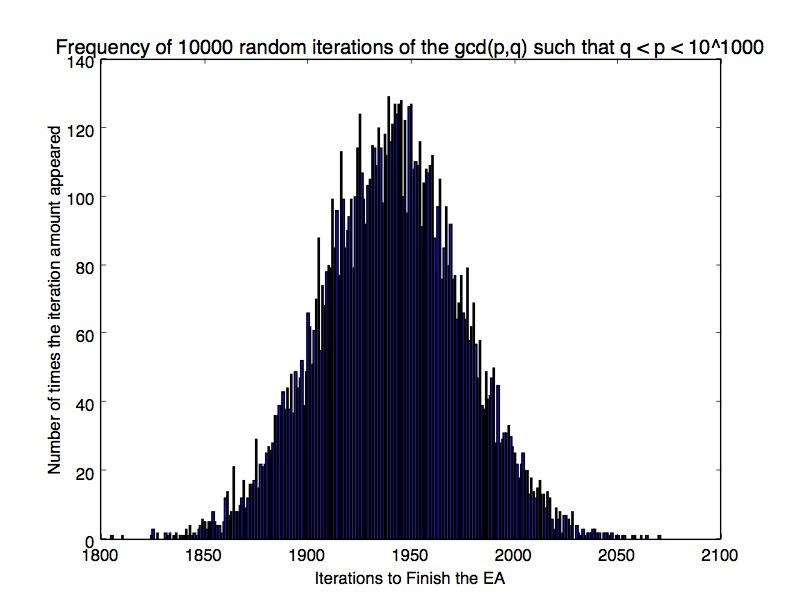
\includegraphics[scale=.3]{1000_digit_numbers.jpg}
		\center \tiny(Figure 5)

\end{frame}

\subsection{Notes}
\begin{frame}
\begin{itemize}
\item in Figure 1, it must be noted that the lack of normality here is due to the lack of available bins. The size of this data set was no more than $4950$, and spanned across merely $9$ bins. As the number of bins needed increases, the more normal the graph becomes.
\item in Figure $5$, the inconsistencies in the normal distribution can be attributed to a too small a sample size. If given the computing power and time, one could compute all pairs less than $10^{1000}$. Note the increasing mean iterations as we climb the upper bound.
\end{itemize}

\end{frame}

\section{Introduction to Complexity Theory}
\begin{frame}
\frametitle{Introduction to Complexity Theory}
\small
\indent Insofar as this course focuses on algorithms, it is first necessary to define the term 'algorithm', as well as several other auxiliary terms used across this presentation.
It is necessary to define some sort of \underline{machine-independent} metric for algorithm running time, so it can be universally used. It is also necessary to define some auxiliary terms to do this:
\begin{itemize}
\item An \underline{algorithm} is a well-defined computational procedure that takes a variable input and halts with an output. (Oorschot and Vanstone, A Handbook of Applied Cryptography)
\item The \underline{running-time} of an algorithm is a function of the number of single-bit operations it takes for an algorithm to complete. 
\item The \underline{size} of an input is the number of bits in the input, or the number of inputs, to an algorithm.
\item The \underline{execution time} of an algorithm's implementation is taken here to mean the average amount of time in nanoseconds for a particular implementation of an algorithm to run. 
\end{itemize}
\end{frame}
\begin{frame}
\frametitle{A Crash Course in Algorithmic Analysis}
\small
\indent Often, the run-time functions can grow to be complex and involve multiple factors. It is often enough to know that a particular algorithm "grows proportionally to" some value (Goodrich, Data Structures and Algorithms in C++). This is known as \underline{asymptotic notation}. \\
\begin{itemize}
\item Let f(n) and g(n) be functions such that $f(n): \mathbb{Z}->\mathbb{R}$ and $g(n): \mathbb{Z}->\mathbb{R}$. Then we say that f(n) is O(g(n)) iff $\exists$ c \textgreater $0$ and n $\in$ $\mathbb{Z}$ such that 
f(n) $\leq$ cg(n), for $\forall$ n' $\geq$ n 
\item This is known as Big-O notation. It allows us to ignore constant factors and lower-order terms, focusing only on the highest-order term--the one which governs its asymptotic behavior.
\item In general, there are six functions fundamental to algorithmic analysis: log(n) \textless n \textless n log(n) \textless $n^2$ \textless $n^3$ \textless $2^n$ (Goodrich, Data Structures and Algorithms in C++)
\item Hence, this is known as asymptotic notation.
\end{itemize}
\end{frame}
\begin{frame}
\frametitle{Bit-Complexity of Integer Operations}
\indent In the ring of integers, we define the bit complexity of addition and multiplication, as well as their inverses, as below: \\ 
\begin{tabular}{|r|l|}
\hline
Operation & Bit-Complexity \\  \hline
+ & O(log(a) + log(b)) = O(log(n)) \\  \hline
- & O(log(a) + log(b)) = O(log(n)) \\ \hline
* & O(log(a) * log(b)) = O($log(n)^2$) \\ \hline
\textbackslash & O(log(a) * log(b)) = O($log(n)^2$) \\ \hline

\end{tabular} \\
\indent These are fundamental values; they allow a baseline computation for running-time complexity. Things like recursion, which incur an extra execution time penalty for function calls, are one of many factors that can confound execution time. \\
\end{frame}
\section{Euclidean Algorithm Variations}
\begin{frame}
\frametitle{Euclidean Algorithm Variations}
\indent Three iterative versions, two recursive versions, and two binary versions of this algorithm were implemented. 
\begin{itemize}
\item Binary GCD algorithm will run with O($log(b)^2$) bit complexity, where b represents the maximum number of bits in the integer inputs.
\item The iterative modular algorithm will run with O(log(u) * log(v)), where u and v are integer inputs. The execution time may be longer, due to an added penalty for function calls.
\item The least-remainders Euclidean algorithm will run in, at the worst case, O(log(u) * log(v)). (Bach and Shallit, Algorithmic Number Theory).
\end{itemize}
\end{frame}
\section{The Algorithms}

\begin{frame}
\frametitle{Iterative, Subtractive}
\begin{algorithm}[H]
\begin{algorithmic}
\STATE{Input: integers U, V}
\STATE{Output: GCD(U,V)}
\IF{ U \textgreater V}
	\STATE{swap(U,V)}
\ENDIF
\WHILE{U $\neq$ V}
	\IF{U \textgreater V}
	\STATE{U <- U - V}
	\ELSE
		\STATE{V = V - U}
	\ENDIF
\ENDWHILE

\STATE{return U}
\end{algorithmic}
\end{algorithm}
\end{frame}

\begin{frame}
\frametitle{Iterative, Modular}
\begin{algorithm}[H]
\begin{algorithmic}
\STATE{Input: integers U, V}
\STATE{Output: GCD(U,V)}
\IF{ V \textgreater U}
	\STATE{swap(U,V)}
\ENDIF
\WHILE{U $\neq$ V}
	\STATE{(U,V) \textless - (V, U MOD V)}
\ENDWHILE
\STATE{return U}
\end{algorithmic}
\end{algorithm}
\indent (Bach and Shallit, Algorithmic Number Theory)
\end{frame}



\begin{frame}
\frametitle{Recursive, Least Remainder}
\begin{algorithm}[H]
\begin{algorithmic}
\STATE{Input: integers U, V}
\STATE{Output: GCD(U,V)}
\IF{ V == 0 }
\STATE{return U}
\STATE{return V}
\ELSE
\STATE{TEMP = V}
\STATE{V = roundMod(U,V)}
\STATE{U = TEMP}
\STATE{return RecursiveEuclidean(V, U MOD V)}
\STATE{return LeastRemainderEuclidean(V, U MOD V)}
\ENDIF

\end{algorithmic}
\\  \hline
\end{frame}

\begin{frame}
\frametitle{Auxiliary Functions for Least Remainder}
\begin{algorithm}[H]
\begin{algorithmic}
\STATE{Input: integers U,V}
\STATE{Output: "Round Mod" function}
\IF{V == 0}
\STATE{return U}
\ELSE
\STATE{Return U = (V * ROUND(U / V))}
\ENDIF
\end{algorithmic}
\end{algorithm}
\end{frame}

\begin{frame}
\begin{algorithm}[H]
\begin{algorithmic}
\STATE{Input: integers U to round}
\STATE{Output: Integer round function}
\STATE{Frac = U - $0.5$}
\STATE{Return CEIL(Frac) as Integer}

\end{algorithmic}
\end{algorithm}
\end{frame}

\begin{frame}
\frametitle{Binary GCD}
\begin{algorithm}[H]
\begin{algorithmic}
\\  \hline
		\STATE{t \textless - abs(U-V)/2}
		\IF{U \textless V}
			\STATE{V \textless - t}
		\ELSE
			\STATE{U \textless - T}
			\STATE{MAX(U,V) = abs(U,V)/2}
		\ENDIF
		\ENDIF		
	\ENDIF
\ENDWHILE
\end{algorithmic}
\end{algorithm}
\end{frame}

\begin{frame}
\frametitle{Binary GCD cont'd}
\begin{algorithm}[H]
\begin{algorithmic}
		\STATE{else}
			\STATE{U \textless - T}
			\STATE{MAX(U,V) = abs(U,V)/2}
		
\STATE{return g*V}

\end{algorithmic}
\end{algorithm}
\end{frame}



\section{Implementation Detail: Java BigInteger Library}
\begin{frame}
\frametitle{Implementation Detail: Java BigInteger Library}
\footnotesize
\begin{itemize} 
\item In order to test these algorithms against large numbers, the Java BigInteger Library was used due to its support for arbitrary-precision arithmetic and numbers.
	\begin{itemize}
	\footnotesize
	\item A BigInteger is an abstraction for an arbitrary-length bit string
	\item In-built GCD function against which our algorithms were compared
	\item No in-built random number generator; used Java's random number 	generator to generate individual bits in a string and wrap these into a 	BigInteger
	\end{itemize}
\item Hierarchical implementation: parent Euclidean Algorithm class with Iterative Algorithm and Recursive Algorithm derived classes; each implementation was a subclass of these
\item In all cases, the corresponding BigInteger arithmetic operation was used; for the binary GCD algorithm, both the arithmetic operations and functions which performed direct bit shifting, were used.
\item All data were collected on a Linux-based server hosted through the Texas A\&M University Department of Computer Science. This process was automated with scripts in Bash.
\end{itemize}
\end{frame}

\section{Baseline Run-Times for BigInteger Library Functions}
\begin{frame}
\frametitle{Baseline Run-Times for BigInteger Library Functions}
\small
\indent In order to effectively measure the running-time of each algorithm, some data on the execution-time of the relevant BigInteger functions were collected, as well as the execution time of our random number generation function: \\
\begin{tabular}{|l|r|}
\hline
Function & Average Time (ns) \\ \hline
Random Number Generation & 1.9e5 ns \\ \hline
Addition & 1.3e5 ns \\ \hline
Subtraction & 1.0e5 ns \\ \hline
Multiplication & 1.4e5 ns \\ \hline
Modulus & 1.4e5 ns \\ \hline
Division & 1.7e5 ns \\ \hline
Left Shift & 3.9e2 ns \\ \hline
Right Shift & 4.7e2 ns \\ \hline
Absolute Value & 2.3e2 ns \\ \hline
Assignment & 2.1e2 ns \\ \hline

\end{tabular}
\small
\\ \indent All data measured was adjusted to account for the costs of absolute value, random number generation, et cetera.
\end{frame}
\section{Complexity Analysis Results}
\begin{frame}
\frametitle{Complexity Analysis Results}
The resultant execution times for each algorithm are given below:

\begin{tabular}{|l|l|}
\hline
	\textbf{Algorithm} & \textbf{Execution Time}
	\\
	\hline Extended & 6.09e9 ns\\
	\hline Iterative, Mod & 4.35e9 ns\\
	\hline Iterative, Subtractive & 1.91e9 ns\\
	\hline Recursive, Mod & 4.77e9 ns\\
	\hline Recursive, Least Positive Remaidner
 & 11.8e9 ns\\
	\hline Stein’s Binary Algorithm, BigInteger Operations & 6.04e9 ns\\
	\hline Stein’s Binary Algorithm, Bit Shifting Operations & 4.68e9 ns\\
	\hline Java BigInteger GCD & 1.30e9 ns\\
	\hline
\end{tabular}

\end{frame}

\begin{frame}
\frametitle{Discussion}
\begin{itemize}
\item A large number of runs for each algorithm were averaged; time elapsed was calculated using the Java System.nanoTime() timer, and adjusted for superfluous costs 
\item Subtractive was among the fastest; lower bitwise cost?
\item Direct bit shifting was also among the fastest; working directly with hardware
\item Number of iterations varied: direct bit shifting was the most expensive bitwise
\item No strong correlation between number of iterations and execution time: least positive remainder is the quickest in terms of iterations, but one of the slower in execution time
\end{itemize}
\end{frame}

\section{Future Work In This Area}
\begin{frame}
\frametitle{Future Work In This Area}
\begin{itemize}
\item All Java programs are run on a virtual machine, allowing a great degree of platform independence; future repetitions will not see a significant change in execution time.
\item Future computational work might consider consolidations of less-expensive bitwise operations rather than consolidations of steps (in the vein of the modulus function)
\item Consider parallel implementations of GCD algorithms
\end{itemize}
\end{frame}



\section{Introduction to Neural Networks}

\begin{frame}
\frametitle{Neural Networks}

Artificial Intelligence (AI) is a growing area in computer science with a myriad of applications across disciplines.  AI is divided into subgroups of study with seven fundamental areas:
\begin{enumerate}
\item reasoning
\item knowledge
\item planning
\item learning
\item communication/natural language processing
\item perception
\item moving and manipulating
\end{enumerate}
As well as an eighth subgroup:
\begin{enumerate}[8.]
\item the notion of distributed intelligence.
\end{enumerate}
\end{frame}

\begin{frame}
\begin{itemize}
\item Machine learning: refers to the ability of a computer to study data, form patterns, and make predictions
\item Typical applications of AI involve pattern-recognition problems; however, applying AI and machine learning methods specifically to number theory problems has not been studied thoroughly
\item Our aim was to evaluate the effectiveness of an Artificial Neural Network when applied to three key problems:
\begin{enumerate}
\item Classification of prime and composite numbers
\item Integer factorization
\item Determining the greatest common divisor (GCD)
\end{enumerate}
\end{itemize}
\end{frame}

\section{Artificial Neural Networks and Their Architecture}
\begin{frame}
\begin{itemize}

\item At its core, an artificial neural network is an abstraction for the functionality of neurons and human cognition
\item The process of learning is achieved through alterations of synaptic connections between neurons, making an ANN the ideal choice for pattern-recognition problems
\end{itemize}
\end{frame}

\subsection{The Neuron}

\begin{frame}

\begin{figure}

	\center 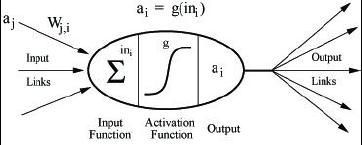
\includegraphics[scale=.8]{neuron_image.jpg}
	\center \tiny(Figure 6)

\end{figure}

\end{frame}

\begin{frame}

\begin{itemize}
\item Input is provided to an input function
\item Each input has an associated weight
\item Each neuron will then compute a weighted sum of its inputs 
\item Then it applies an activation function to act as a threshold to derive output
\end{itemize}

\end{frame}

\begin{frame}

There are several options for Thresholding Functions:

\begin{itemize}
\item AND
\item OR
\item XOR
\item Linear
\item Sigmoid
\item Hyperbolic Tangent 
\end{itemize}

The complexity of the problem being attempted by the ANN determines the correct function to use.

\end{frame}

\begin{frame}
\begin{itemize}
\item Neurons whose activation functions create hard thresholds are called perceptrons.  
\item Neurons whose activation functions are logistic functions are known as sigmoid perceptrons.
\item The perceptron maps input directly to output.
\item Historically, single perceptrons were used to solve problems, but were not nearly as successful.
\end{itemize}
\end{frame}

\begin{frame}
There are two principal ANN architectures:
\begin{enumerate}
\item Feed-forward networks
\begin{itemize}
\item Directed, acyclic graph
\item Flows in one direction only
\item It maintains no internal state nor represents more than the input passed to the network
\item May be split into multiple layers: Input, Hidden, Output
\item Lacks any kind of memory
\end{itemize}
\item Recurrent Networks
\begin{itemize}
\item Utilizes the notion of recurrence 
\item Cyclic
\item Maintains a small amount of short-term memory
\end{itemize}
\end{enumerate}

\end{frame}

\begin{frame}
There are two main learning methods in an ANN:
\begin{enumerate}
\item Supervised
\begin{itemize}
\item Done through an external teacher
\item The network is told the desired response to certain input signals
\item Reinforcement learning is a form of supervised where a correct response is given a certain weight and the better the weight, the more correct the answer
\end{itemize}

\item Unsupervised
\begin{itemize}
\item Also known as self-organizing
\item Based entirely upon local information
\item The network is given a large amount of data and allowed to recognize its own patterns
\end{itemize}
\end{enumerate}
\end{frame}

\begin{frame}
Implementation of any learning algorithm, supervised or unsupervised, is complicated by the presence of multiple outputs and hidden layers of the network: the fact that the hidden layer leaves its computations out of reach of the user means that any information obtained about errors at the hidden layer is all but useless to the user. Therefore, an algorithm for backpropagation must be used to back-propagate errors from the output layer to hidden layers.
\end{frame}

\begin{frame}
\begin{figure}
	\center 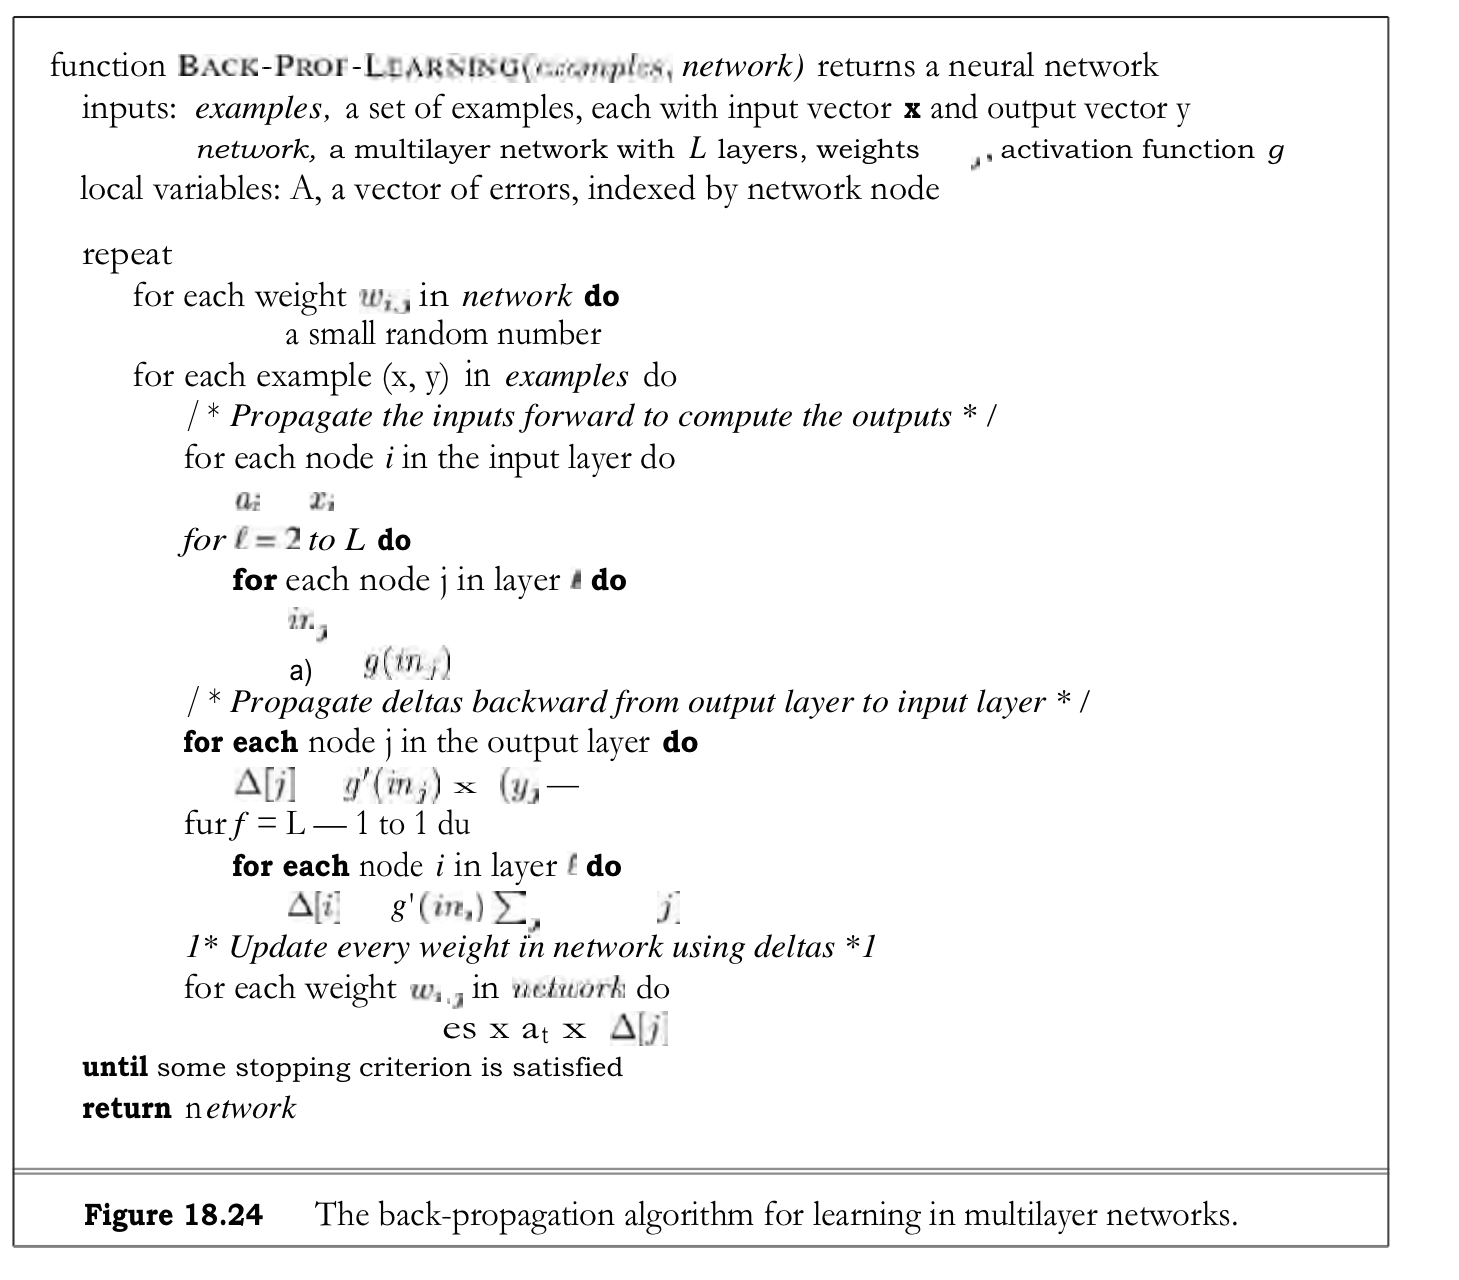
\includegraphics[scale=.195]{backprop.png}
	\center \tiny(Figure 7)
\end{figure}
\end{frame}


\section{Attempts at using Neural Networks}
\begin{frame}
The ANN was implemented in Python, using the Pybrain machine learning library.
The network was set up as a reinforced back-propagation system.
For factorization, a class was defined containing prime factorizations of numbers 1 through 15.
For primality testing, a list of prime numbers up to 10,000 was obtained.
For the GCD problem, numbers were randomly generated from 0 to 100, and every possible combination of pairs tested.
\end{frame}

\begin{frame}
The teaching dataset used was combinations of ($x$,$y$), with $x$ ranging from $2$-$5$ and $y$ ranging from $1$-$20$.  
The input was a pair of $x$ and $y$ combined with the desired output of the gcd.  It was set up to randomly go through $10,000$ iterations of the training dataset and then attempt to guess the output for each of the teaching entries.
For the majority of the runs, there were $2$ hidden layers activated.
When the learning rate was increased from $0.05$ to $0.1$, the results improved slightly, though not drastically.
Momentum was determined to work best at the value $0.025$.
Surprisingly, the organization of the training data had some of the most interesting results.
\end{frame}

\begin{frame}
Sample data:
(2,1) [ 1.]
(2,2) [ 2.]
(2,3) [ 1.58476845]
\newline (2,4) [ 1.58827758]
(2,5) [ 1.58827945]
(2,6) [ 1.58827945]
\newline (2,7)  [ 1.58827945]
(2,8) [ 1.58827945]
(2,9) [ 1.58827945]
\newline (2,10)  [ 1.58827945]
(3,1) [ 0.99940695]
(3,2) [ 1.00206377]
\newline (3,3) [ 3.38776544]
(3,4) [ 1.58842719]
(3,5) [ 1.58827903]
\newline (3,6) [ 1.58827945]
(3,7) [ 1.58827945]
(3,8) [ 1.58827945]
\newline (3,9) [ 1.58827945]
(3,10) [ 1.58827945]
(4,1) [ 0.99940584]
\newline (4,2) [ 0.99941081]
(4,3) [ 1.01127187]
(4,4) [ 4.41099692]
\newline (4,5) [ 1.58941163]
(4,6) [ 1.58827936]
(4,7) [ 1.58827945]
\newline (4,8) [ 1.58827945]
(4,9) [ 1.58827945]
(4,10) [ 1.58827945]
\newline (5,1) [ 0.99940584]
(5,2) [ 0.99940585]
(5,3) [ 0.99942807]
\newline (5,4) [ 1.05195013]
(5,5) [ 4.77198339]
\end{frame}

\section{Neural Networks Results}

\begin{frame}
There are several explanations that could be applied to why the network was unable to produce the desired results.
\begin{enumerate}
\item The training dataset could have been too small.
\item Prime numbers do not follow a well-defined pattern.
\item Only feed-forward networks were used.
\item Not all potential functions for activation were tested.
\item While various parameters of the network were tested, very little was tested in the way of data representation beyond an elementary normalization of GCD inputs and outputs.
\item Finally, it could be that a neural network in the implementation used for our project is simply not well suited for this type of problem.
\end{enumerate}
\end{frame}

\begin{frame}
There have already been well established algorithms, as demonstrated in the previous project, which rely on more concrete building blocks than just recognizing patterns that may not even be there. It is possible that other methods of artificial intelligence, such as support vector machines, might have more success at one or all of the problems investigated.
\end{frame}




\section{References}
\begin{frame}
\frametitle{References}
\footnotesize{
\begin{thebibliography}{99} % Beamer does not support BibTeX so references must be inserted manually as below
\bibitem[Epasinghe, 1983]{p1} P. W. Epasinghe (1983)
\newblock Euclid's Algorithm and the Fibonacci Numbers
\newblock \emph{The Fibonacci Quarterly}

\bibitem[Bach, Jeffery]{p2} Bach, Eric and Jeffrey Shallit (1996)
\newblock Algorithmic Number Theory
\newblock \emph{Foundations of Computing Series}

\bibitem[]{p3} Menezes, A.J., van Oorschot, P. and Scott Vanstone (1997)
\newblock Handbook of Applied Cryptography
\newblock \emph{CRC Press}
\end{thebibliography}
}
\end{frame}

%------------------------------------------------
\section{End}
\begin{frame}
\Huge{\centerline{The End}}
\end{frame}

%----------------------------------------------------------------------------------------

\end{document} 